%=====================================================================
\section{Results I: the 2026 disclosure shock}\label{sec:shock}

Figure~\ref{fig:volume} shows that CVE publication grew steadily from about 6,500 a year in 2015--2016 to 39,924 in 2024 and 48,150 in 2025. It then broke trend in 2026. Between January and October 2026, 89,845 CVEs were published, 2.27 times the 39,638 published over the same months of 2025. Monthly volume rose from 4,274 in October 2025 to 17,051 in October 2026, and the acceleration began around March 2026. By 12 November, 96,498 CVEs had been published in 2026.

\begin{figure}[!htbp]
\centering
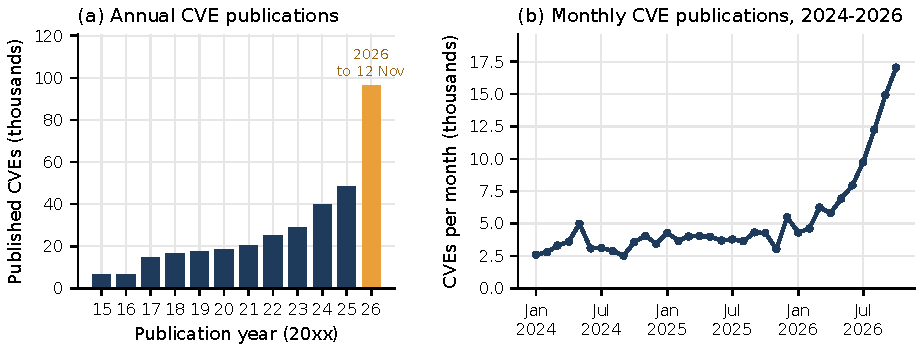
\includegraphics[width=\textwidth]{fig02_cve_volume.pdf}
\caption{CVE publication volume. (a) Annual totals; the 2026 bar covers 1 January to 12 November. (b) Monthly totals, January 2024 to October 2026. Source: CVE List V5 snapshot, author calculations.}
\label{fig:volume}
\end{figure}

The surge is not confined to open-source projects. Table~\ref{tab:vendor} and Figure~\ref{fig:vendor} show that vulnerabilities assigned by large commercial vendors' own CNAs rose by factors of 33 (Google Chrome), 13 (Oracle), 4 (Microsoft) and 2 (Apple). For banks, this matters more than the total: these vendors supply the browsers, operating systems, office software, databases and middleware on which every bank runs. The patch workload of a bank's IT function scales with these counts. A doubling or quadrupling of vendor advisories in a single year is an operational shock even before any vulnerability is exploited.

\begin{figure}[!htbp]
\centering
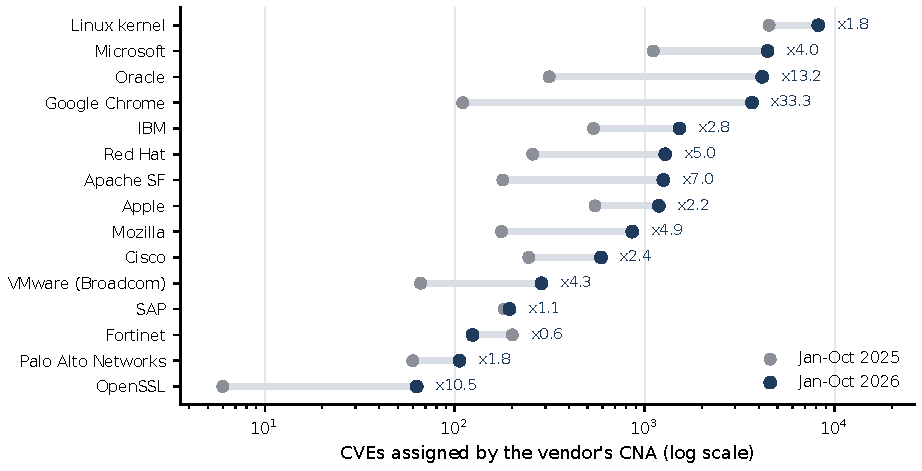
\includegraphics[width=\textwidth]{fig03_vendor_surge.pdf}
\caption{CVEs assigned by selected CNAs, January--October 2025 vs.\ January--October 2026 (log scale). Labels show the ratio.}
\label{fig:vendor}
\end{figure}

\begin{table}[!htbp]
\centering
\caption{CVE counts by assigning CNA, January--October, with credit coverage and AI-credited CVEs in 2026.}
\label{tab:vendor}
\small
\begin{tabular}{lrrrrr}
\toprule
Assigning CNA & Jan--Oct 2025 & Jan--Oct 2026 & Ratio & Credited (\%) & AI-credited \\
\midrule
Linux kernel & 4,516 & 8,197 & 1.8 & 0 & 0 \\
Microsoft & 1,108 & 4,437 & 4.0 & 0 & 0 \\
Oracle & 314 & 4,154 & 13.2 & 0 & 0 \\
Google Chrome & 110 & 3,667 & 33.3 & 0 & 0 \\
IBM & 538 & 1,524 & 2.8 & 15 & 1 \\
Red Hat & 257 & 1,282 & 5.0 & 73 & 176 \\
Apache SF & 179 & 1,252 & 7.0 & 90 & 177 \\
Apple & 547 & 1,187 & 2.2 & 0 & 0 \\
Mozilla & 176 & 859 & 4.9 & 100 & 95 \\
Cisco & 245 & 589 & 2.4 & 17 & 0 \\
VMware (Broadcom) & 66 & 286 & 4.3 & 5 & 0 \\
SAP & 182 & 194 & 1.1 & 0 & 0 \\
Fortinet & 201 & 124 & 0.6 & 0 & 0 \\
Palo Alto Networks & 60 & 106 & 1.8 & 97 & 1 \\
OpenSSL & 6 & 63 & 10.5 & 100 & 30 \\
\bottomrule
\end{tabular}
\end{table}

\paragraph{What caused the shock?} The data cannot attribute the surge to AI on their own. The CNAs with the largest increases (Microsoft, Chrome, Oracle) publish no credits, so their records do not say who or what found the bugs. Three observations nevertheless point to AI-assisted discovery as a major contributor. First, the timing coincides with the deployment of agentic security researchers and restricted-access defensive programmes in late 2025 and 2026 \citep{openai2025aardvark,deepmind2025codemender,anthropic2026glasswing}. Second, among CNAs that do publish credits, AI-credited records rose from almost none to hundreds per month over the same period (Section~\ref{sec:ai}). Third, the CNAs that publish credits and grew fastest---Apache (+177 AI-credited CVEs in 2026), Red Hat (+176), Mozilla (+95) and OpenSSL (+30)---have substantial AI-credited shares. Other factors, including CNA process changes and the expansion of CNAs such as VulnCheck and GitHub, also contribute. We treat AI as a likely but unquantified driver of the commercial-vendor surge.

%=====================================================================
\section{Results II: AI in vulnerability discovery}\label{sec:ai}

\subsection{Scale and trajectory}
We identify 1,598 AI-credited CVEs: 665 in Tier~1 (an AI system named) and 933 in Tier~2 (an AI-native organisation credited). Seven appear before 2025, 151 in 2025 and 1,440 in 2026. The first Tier~1 credit in our data is dated 20 March 2025 (XBOW, an autonomous penetration-testing system, credited on an Apache CVE). Figure~\ref{fig:aimonthly} shows that monthly counts grew at about 18.6\% per month (s.e.\ 3.8 percentage points) between July 2025 and October 2026, a doubling time of about 4.1 months. In October 2026, AI-credited CVEs were 4.1\% of all CVEs that carry any credit and 2.0\% of all CVEs. Because the largest commercial CNAs publish no credits, the true share is higher.

\begin{figure}[!htbp]
\centering
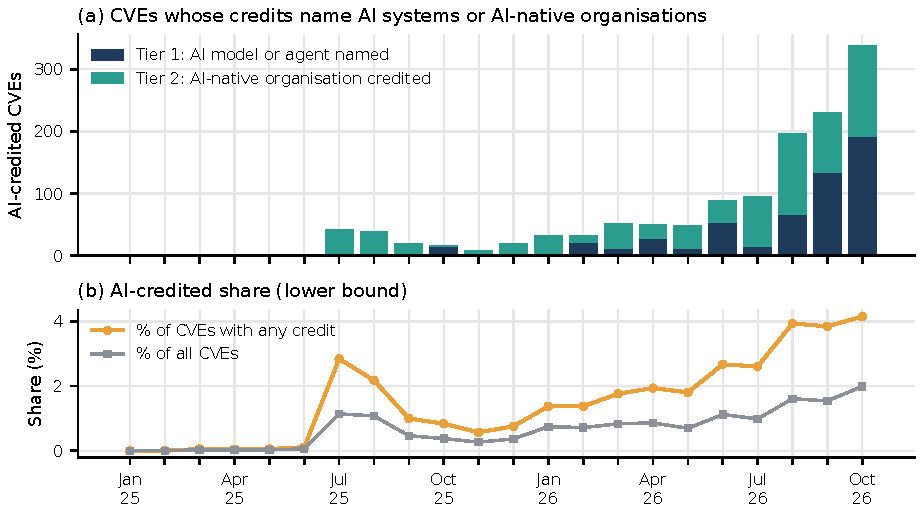
\includegraphics[width=\textwidth]{fig04_ai_monthly.pdf}
\caption{AI-credited CVEs per month, January 2025 to October 2026. (a) Counts by tier. (b) Share of CVEs with any credit, and share of all CVEs. Both shares are lower bounds.}
\label{fig:aimonthly}
\end{figure}

\subsection{Who is credited and what they find}
Table~\ref{tab:developers} and Figure~\ref{fig:aibreak}(a) show a concentrated field. Credits naming Anthropic's Claude models and agents (510) and the AI-native firm AISLE (438) dominate, followed by OpenAI (196, of which 74 name Codex Security or a GPT model), ZAST.AI (171) and a long tail of smaller AI security firms. Google's Big Sleep appears on 18 CVEs. These include CVE-2025-6965 in SQLite, which the vendor described as otherwise known only to threat actors---an example of AI \emph{pre-empting} exploitation (Table~\ref{tab:milestones}).

\begin{table}[!htbp]
\centering
\begin{minipage}[t]{0.45\textwidth}
\centering
\caption{AI-credited CVEs by credited developer. A CVE can credit more than one developer.}
\label{tab:developers}
\small
\resizebox{\textwidth}{!}{\begin{tabular}{lrrr}
\toprule
Developer credited & Tier 1 & Tier 2 & Total \\
\midrule
Anthropic & 510 & 0 & 510 \\
AISLE & 0 & 438 & 438 \\
OpenAI & 74 & 122 & 196 \\
ZAST.AI & 0 & 171 & 171 \\
Other AI tools/orgs & 74 & 28 & 102 \\
WatchGuard & 0 & 28 & 28 \\
Striga & 0 & 28 & 28 \\
depthfirst & 0 & 22 & 22 \\
Horizon3.ai & 0 & 21 & 21 \\
Mopmonk AI & 0 & 20 & 20 \\
Google & 18 & 0 & 18 \\
CodeAnt AI & 0 & 18 & 18 \\
Other (7 developers) & 8 & 49 & 57 \\
\bottomrule
\end{tabular}}
\end{minipage}\hfill
\begin{minipage}[t]{0.52\textwidth}
\centering
\caption{Severity of 2026 CVEs by credit type (maximum CVSS base score where available).}
\label{tab:severity}
\small
\resizebox{\textwidth}{!}{\begin{tabular}{lrrrr}
\toprule
Group (CVEs published in 2026) & Scored & Mean CVSS & High+ (\%) & Critical (\%) \\
\midrule
AI-credited (tier 1) & 593 & 7.07 & 56.8 & 9.8 \\
AI-credited (tier 2) & 796 & 6.83 & 47.6 & 9.0 \\
Human-credited & 40,338 & 6.98 & 51.3 & 12.4 \\
All other 2026 CVEs & 89,689 & 7.07 & 56.8 & 12.4 \\
\bottomrule
\end{tabular}}
\vspace{4pt}
\parbox{\textwidth}{\footnotesize Mann--Whitney test, all AI-credited vs.\ human-credited: $p=0.66$.}
\end{minipage}
\end{table}

\begin{figure}[!htbp]
\centering
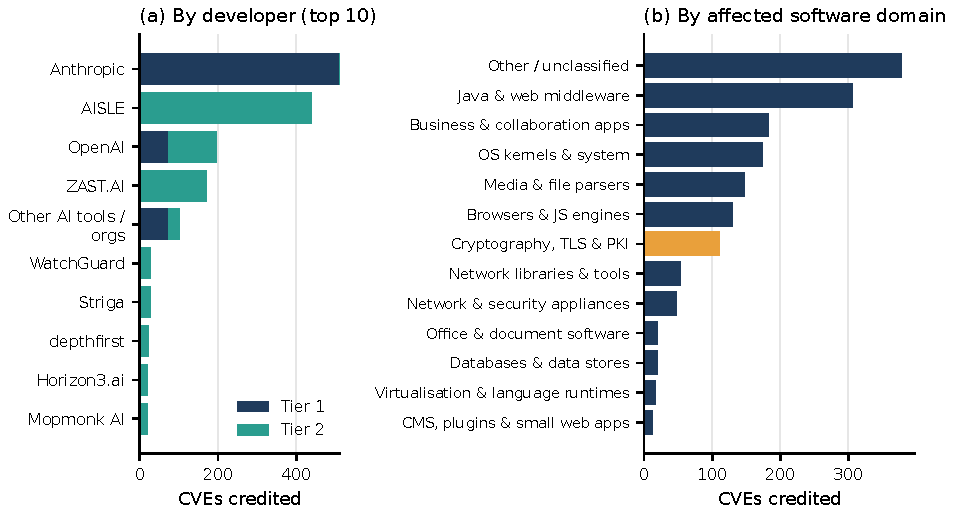
\includegraphics[width=\textwidth]{fig05_ai_breakdown.pdf}
\caption{AI-credited CVEs (a) by credited developer (top 10) and (b) by affected software domain. Cryptography, TLS and PKI libraries are highlighted.}
\label{fig:aibreak}
\end{figure}

The affected software is mostly open-source infrastructure: Java and web middleware (largely Apache projects), operating-system components, media parsers, browsers, and business and collaboration applications (Figure~\ref{fig:aibreak}b). One domain stands out for banking: 111 AI-credited CVEs affect cryptographic, TLS and PKI libraries. These comprise 52 in Bouncy Castle, the dominant Java cryptography provider in enterprise and banking software; 33 in OpenSSL; and 25 in wolfSSL/wolfSSH, which is widely embedded in devices. Cryptographic libraries are the software layer of the trust anchors discussed in Section~\ref{sec:hardware}.

\paragraph{Severity.} AI-credited vulnerabilities are not trivial. In 2026, Tier~1 CVEs had a mean maximum CVSS score of 7.07, with 56.8\% rated high or critical, against 6.98 and 51.3\% for human-credited CVEs (Table~\ref{tab:severity}). The difference between all AI-credited and human-credited CVEs is not significant ($p=0.66$). AI systems find vulnerabilities of the same severity as human researchers.

\subsection{From AI discovery to exploitation}
Fifteen AI-credited CVEs have entered the KEV catalogue (Table~\ref{tab:aikev}). Three features stand out. First, the median lag from publication to KEV listing is 17 days; these were exploited as n-days after disclosure rather than as zero-days. Second, seven of the fifteen were found by Horizon3.ai, an offensive-security firm that focuses on enterprise products attackers prize, so the apparent exploitation rate of AI-credited CVEs (9.4 per 1,000, against 1.5 for human-credited CVEs over 2023--2026) reflects \emph{what} these firms look at more than \emph{how} they find it. Third, only one Tier~1 CVE (Brotli, credited to OpenAI Codex Security) has been exploited, and none of the 86 Tier~1 CVEs in the censoring-robust cohort was listed within 180 days. Products in this set---SolarWinds Web Help Desk, SimpleHelp, JFrog Artifactory, Apache ActiveMQ and Tomcat, Palo Alto Expedition, Langflow and PHP---are typical of enterprise estates, including banks.

\begin{table}[!htbp]
\centering
\caption{AI-credited CVEs that entered the KEV catalogue.}
\label{tab:aikev}
\scriptsize
\resizebox{\textwidth}{!}{\begin{tabular}{llllrr}
\toprule
CVE & Product & Credited AI party & Published & KEV listed & Lag (d) \\
\midrule
CVE-2023-27524 & Apache Superset & Horizon3.ai & 2023-04-24 & 2024-01-08 & 259 \\
CVE-2024-9465 & Palo Alto Networks Expedition & Horizon3.ai & 2024-10-09 & 2024-11-14 & 36 \\
CVE-2025-3248 & Langflow Langflow & Horizon3.ai & 2025-04-07 & 2025-05-05 & 28 \\
CVE-2025-5086 & Dassault Systèmes DELMIA Apriso & Hacktron & 2025-06-02 & 2025-09-11 & 101 \\
CVE-2025-40551 & SolarWinds Web Help Desk & Horizon3.ai & 2026-01-28 & 2026-02-03 & 6 \\
CVE-2025-40536 & SolarWinds Web Help Desk & Horizon3.ai & 2026-01-28 & 2026-02-12 & 15 \\
CVE-2026-34197 & Apache ActiveMQ & Horizon3.ai & 2026-04-07 & 2026-04-16 & 9 \\
CVE-2026-48558 & SimpleHelp  SimpleHelp & Horizon3.ai & 2026-06-12 & 2026-06-29 & 17 \\
CVE-2026-34486 & Apache Tomcat & Striga & 2026-04-09 & 2026-08-04 & 117 \\
CVE-2026-66384 & JFrog Artifactory & OpenAI (organisation) & 2026-08-12 & 2026-08-27 & 15 \\
CVE-2026-42016 & JFrog Artifactory & OpenAI (organisation) & 2026-07-27 & 2026-09-11 & 46 \\
CVE-2026-5430 & WSO2 Multiple Products & Hacktron & 2026-08-06 & 2026-09-24 & 49 \\
CVE-2026-109618 & PHP Group PHP & OpenAI (organisation) & 2026-10-21 & 2026-10-26 & 5 \\
CVE-2026-109619 & PHP Group PHP & OpenAI (organisation) & 2026-10-21 & 2026-10-26 & 5 \\
CVE-2026-111497 & Google Brotli & Codex Security / Aardvark & 2026-10-22 & 2026-10-27 & 5 \\
\bottomrule
\end{tabular}}
\end{table}

\paragraph{Answer to RQ1.} AI-credited discovery went from negligible to roughly 2--4\% of credited CVEs in eighteen months and is doubling every four months. The publicly visible activity is overwhelmingly defensive or coordinated: AI developers, AI-native security firms and open-source maintainers disclosing and fixing bugs. Offensive use is documented in threat reports \citep{microsoft2024threat,anthropic2025espionage}, but does not appear in vulnerability records, because attackers do not credit themselves. The number of people ``using AI to hunt for zero-days'' therefore cannot be counted directly. The observable footprint is large and growing, and the capability it reveals is available, with some lag, to attackers.

%=====================================================================
\section{Results III: exploitation of commercial software}\label{sec:exploitation}

\subsection{What gets exploited}
Of the 1,779 KEV entries, 263 vendors appear among additions since 2022; the ten most frequent (led by Microsoft, Cisco, Adobe, Apple, Google and Oracle) account for 51.8\%. Figure~\ref{fig:kevcat} shows how the composition of additions has shifted. Enterprise perimeter and network infrastructure---VPN, firewall, application-delivery and router platforms from vendors such as Fortinet, Palo Alto Networks, Citrix, Ivanti, Cisco and SonicWall---rose from 14.6\% of additions in 2022 to 21.0\% in 2026. IT-management and remote-access tools rose to 14.6\% in 2026, from 1.8\% in 2022. Browsers and plug-ins declined. A new category appeared: AI and automation platforms (for example Langflow and LiteLLM), with 12 entries, 11 of them added in 2026. The Herfindahl index of exploitation across vendors fell from 0.114 in 2022 to 0.035 in 2026: attackers now exploit a wider range of vendors.

\begin{figure}[!htbp]
\centering
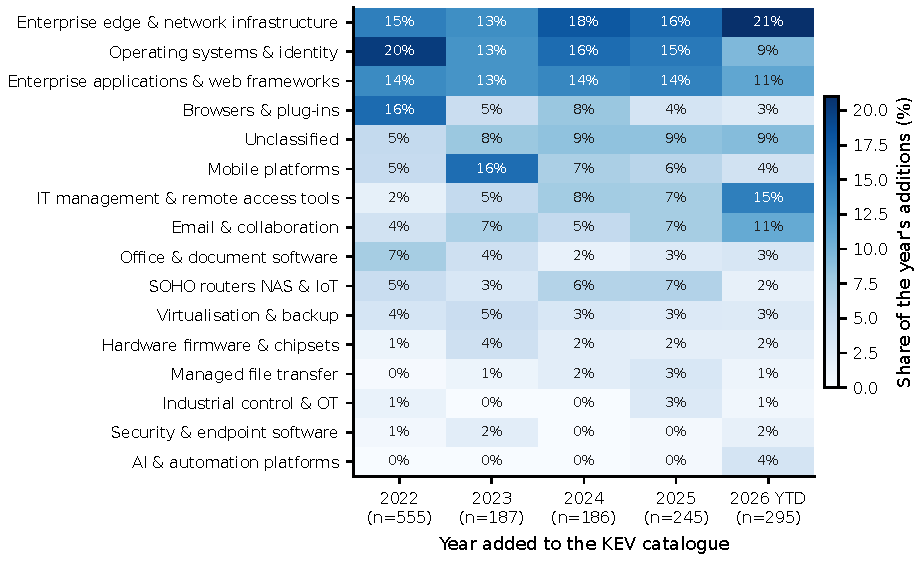
\includegraphics[width=\textwidth]{fig06_kev_categories.pdf}
\caption{Composition of KEV additions by product category and year (share of the year's additions). 2021 is omitted because the catalogue launched with a back-filled list.}
\label{fig:kevcat}
\end{figure}

\subsection{How fast exploitation follows disclosure}
Table~\ref{tab:lags} and Figure~\ref{fig:lags}(a) report listing lags. In the censoring-robust cohort, the median lag has been between 4 and 6 days for every publication year since 2022. Between 51.5\% and 64.9\% of listed vulnerabilities were listed within a week, and 28--39\% were listed on or before the day the CVE was published. We find no further compression after 2022 (Kendall's $\tau=0.035$, $p=0.20$). Industry studies report that the average time-to-exploit fell from about a month to a few days during 2021--2023 \citep{mandiant2024tte}; our data suggest that the compression has since plateaued at that low level. This does not support the stronger form of our hypothesis H2 (continuing compression). The weaker form holds: the window is already too short for monthly patch cycles.

\begin{table}[!htbp]
\centering
\caption{KEV listing lags by CVE publication year (censoring-robust cohort), and zero-day proxy counts vs.\ published industry counts.}
\label{tab:lags}
\small
\begin{tabular}{lrrrrrrr}
\toprule
 & \multicolumn{5}{c}{Cohort: listed within 180 days} & \multicolumn{2}{c}{Zero-day counts} \\
\cmidrule(lr){2-6}\cmidrule(lr){7-8}
CVE year & $n$ & Median lag & IQR & $\le 0$ d (\%) & $\le 7$ d (\%) & Proxy & Reported \\
\midrule
2021$^a$ & 16 & 20.0 & [0, 143] & 31.2 & 50.0 & 8 & -- \\
2022 & 99 & 6.0 & [-1, 45] & 39.4 & 51.5 & 51 & 55 \\
2023 & 134 & 4.0 & [0, 14] & 34.3 & 64.9 & 87 & 97 \\
2024 & 132 & 4.5 & [0, 36] & 29.5 & 59.1 & 78 & 75 \\
2025 & 175 & 5.0 & [0, 33] & 28.0 & 55.4 & 97 & -- \\
2026$^b$ & 65 & 5.0 & [0, 15] & 27.7 & 56.9 & 128 & -- \\
\bottomrule
\end{tabular}
\vspace{2pt}
\parbox{0.95\textwidth}{\footnotesize $^a$~November--December 2021 only. $^b$~CVEs published to mid-May 2026. ``Proxy'' counts all early-listed post-launch entries by publication year. ``Reported'': industry counts of in-the-wild zero-days as reported by Mandiant (2022) and Google (2023, 2024) \citep{mandiant2023zeroday,google2024zeroday,gtig2025zeroday}. Google Project Zero's own count for 2022 was 41. Benchmark figures should be verified against the original reports.}
\end{table}

\begin{figure}[!htbp]
\centering
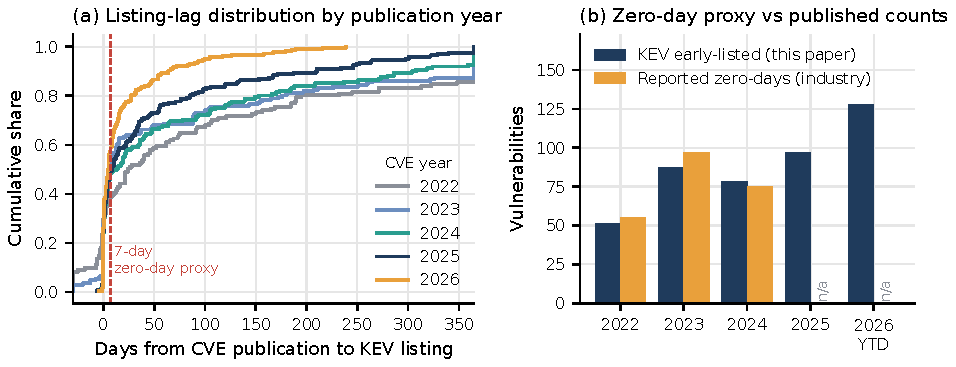
\includegraphics[width=\textwidth]{fig07_lags.pdf}
\caption{(a) Cumulative distribution of days from CVE publication to KEV listing, by publication year (clipped to $[-30,365]$). (b) Annual count of early-listed vulnerabilities (zero-day proxy) vs.\ industry-reported zero-day counts.}
\label{fig:lags}
\end{figure}

\paragraph{Validating the zero-day proxy.} Early-listed counts by publication year were 51, 87 and 78 for 2022--2024, against reported in-the-wild zero-day counts of 55, 97 and 75---a mean absolute deviation of 7.2\% (Figure~\ref{fig:lags}b). The two series measure overlapping but not identical sets, so the agreement supports using the proxy for levels and trends, not for individual classification. On this proxy, zero-day-like exploitation rose to 97 in 2025 and 128 in 2026 to date, the highest in the series.

\subsection{Exploitation has grown more slowly than discovery}
KEV additions rose from 186 in 2024 to 245 in 2025 and 295 in 2026 to 10 November. Disclosure grew much faster, so the share of new CVEs that are exploited fell (Table~\ref{tab:k180}). In the censoring-robust cohort, an average of 3.89 of every 1,000 CVEs published between 2022 and 2025 were listed within 180 days, against 2.62 per 1,000 in the first half of 2026. If the disclosure shock is substantially AI-driven, the defenders' side of AI is currently ahead: vulnerabilities are being found and fixed faster than attackers are converting them into exploitation. This is our hypothesis H1. The same numbers carry a warning. A falling exploitation \emph{rate} on a quadrupling \emph{base} still means more exploited vulnerabilities in absolute terms, and the defenders' patch workload has multiplied.

\begin{table}[!htbp]
\centering
\caption{KEV listings within 180 days per 1,000 CVEs, by publication half-year.}
\label{tab:k180}
\small
\begin{tabular}{lrrr}
\toprule
Publication half-year & CVEs & In KEV within 180 d & Per 1,000 \\
\midrule
2022H1 & 12,343 & 53 & 4.29 \\
2022H2 & 12,656 & 46 & 3.63 \\
2023H1 & 14,120 & 55 & 3.90 \\
2023H2 & 14,727 & 79 & 5.36 \\
2024H1 & 20,349 & 54 & 2.65 \\
2024H2 & 19,575 & 78 & 3.98 \\
2025H1 & 23,642 & 96 & 4.06 \\
2025H2 & 24,508 & 79 & 3.22 \\
2026H1 & 24,815 & 65 & 2.62 \\
\bottomrule
\end{tabular}
\end{table}

\paragraph{Answer to RQ2.} The commercial products exploited most often, and most often as zero-days, are perimeter devices (59.9\% zero-day-like), operating systems (61.8\%), browsers (93.2\%), mobile platforms (70.8\%) and managed file transfer (64.7\%). Products with the heaviest ransomware association are mail and collaboration servers (37.2\%), MFT (35.3\%) and IT-management tools (29.3\%) (Table~\ref{tab:profile}). Well-known named campaigns in these categories---MOVEit, GoAnywhere, Accellion FTA, Exchange ProxyLogon, Citrix NetScaler, Ivanti Connect Secure, Fortinet FortiOS, SharePoint and Oracle E-Business Suite---are the specific products behind these aggregates.

%=====================================================================
\section{Hardware trust anchors and hardware wallets}\label{sec:hardware}

RQ3 asks whether zero-days in hardware wallets matter for banks. Table~\ref{tab:hardware} summarises 11 cases. Hardware wallets share their building blocks with banking infrastructure: secure elements, microcontrollers, firmware and cryptographic libraries. These same blocks protect payment cards, PIN and payment HSMs, FIDO keys used by bank staff, TPMs in servers, and the secure enclaves of the phones that run mobile banking.

\begin{table}[!htbp]
\centering
\caption{Hardware trust-anchor cases and their banking analogues (author-coded from public research and reporting).}
\label{tab:hardware}
\scriptsize
\begin{tabular}{p{0.05\textwidth}p{0.19\textwidth}p{0.24\textwidth}p{0.16\textwidth}p{0.24\textwidth}}
\toprule
Year & Target & Attack class & Access required & Banking analogue \\
\midrule
2010 & EMV chip-and-PIN cards & Protocol logic flaw (PIN verification bypass) & Physical card and modified terminal & Card-present payments \\
2017 & Infineon RSA key generation (ROCA) & Weak key generation (factorable public keys) & Remote (public key only) & Smart cards; tokens; TPMs; national ID used for e-banking \\
2018 & Trezor; Ledger; KeepKey (wallet.fail) & Fault injection and supply-chain tampering & Physical device & Hardware authentication tokens; HSM tamper resistance \\
2019 & Apple BootROM A5-A11 (checkm8) & Unpatchable BootROM memory-safety bug & Physical (USB) & Integrity of phones running mobile banking \\
2019 & General-purpose HSM (research disclosure) & Firmware memory-safety bugs enabling key extraction & Network/API access to HSM & Payment and PIN HSMs in bank data centres \\
2019 & Intel fTPM and STMicro TPM (TPM-Fail) & Timing side channel on ECDSA & Local or network timing & Server attestation and key storage \\
2020 & Trezor One/T seed extraction & Voltage glitching of microcontroller & Physical (minutes) & Stolen token or HSM scenarios \\
2021 & EMV contactless (Visa PIN bypass) & Protocol flaw allowing PIN bypass & Physical proximity (relay) & Contactless payments \\
2023 & Ledger Connect Kit & Malicious library version published via compromised account & Remote & Banking SDKs and front-end libraries \\
2024 & Infineon ECDSA in YubiKey 5 (EUCLEAK) & Electromagnetic side channel & Physical (lab equipment) & FIDO keys used by bank staff \\
2025 & Bybit cold-wallet signing (Safe interface) & Manipulated transaction display (blind signing) & Remote (supplier compromise) & Maker-checker payment approval screens \\
\bottomrule
\end{tabular}
\end{table}

Three lessons follow. First, six of the eleven cases require physical access to the device: glitching, side channels, or a USB connection to a boot ROM. Such attacks do not scale to a remote campaign against a bank, but they matter for stolen tokens, insider threats and supply-chain tampering. Second, the remote cases are the dangerous ones, and they sit in software around the hardware. ROCA was a flaw in key generation in a secure-element library, exploitable from a public key alone \citep{nemec2017roca}. The Ledger Connect Kit incident was a compromised software dependency. The 2025 Bybit theft manipulated the transaction-display layer of a multisig signing workflow, so that signers approved a transfer they did not intend. The banking analogue of this last case is the maker--checker approval screen for high-value payments. Third, AI discovery is now active in exactly this software layer: 111 AI-credited CVEs affect cryptographic libraries (Section~\ref{sec:ai}).

\paragraph{Answer to RQ3.} Hardware-wallet zero-days are relevant to banks less through the wallets themselves than through common components and patterns. These are secure-element libraries (ROCA-type flaws), HSM firmware \citep{campana2019hsm}, payment-card protocols \citep{murdoch2010chip,basin2021emv} and transaction-display integrity in signing workflows. Banks and central banks that hold or plan to hold digital assets, issue tokenised deposits or pilot CBDC with offline hardware wallets inherit these risks directly.

%=====================================================================
\section{Financial-sector exposure}\label{sec:exposure}

\subsection{Bank-weighted exploitation pressure}
Weighting KEV categories by their relevance to bank estates (Figure~\ref{fig:pressure}, Table~\ref{tab:profile}) puts enterprise perimeter infrastructure first ($\Pi=162$, of which 97 zero-day-like), followed by operating systems and identity (91.7), enterprise applications and web frameworks (81.6), IT-management and remote-access tools (73.8), and mail and collaboration (70.2). The ranking is robust to the weights: across 2,000 random perturbations of $\pm0.3$, the median Kendall rank correlation with the baseline is 0.88 (5th percentile 0.80), and it is 0.83 under uniform weights.

\begin{figure}[!htbp]
\centering
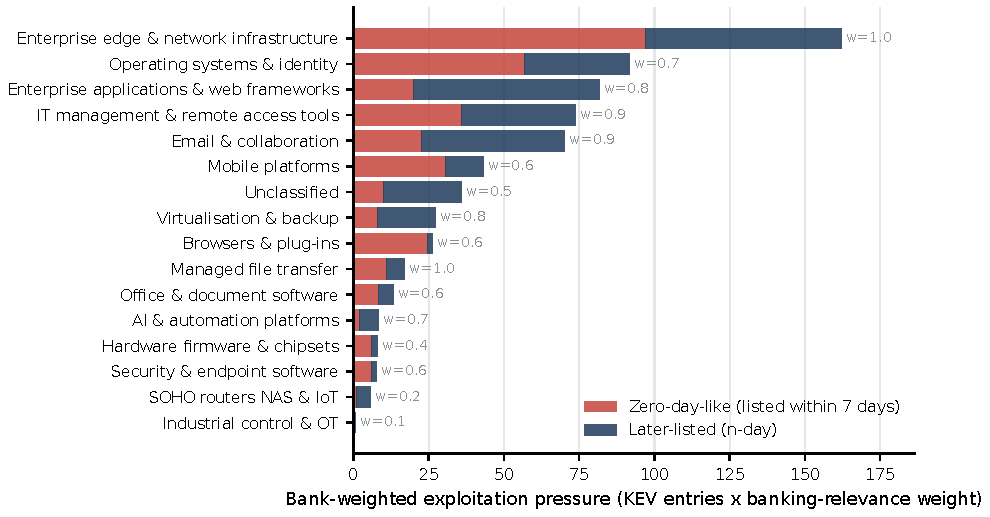
\includegraphics[width=\textwidth]{fig08_bank_pressure.pdf}
\caption{Bank-weighted exploitation pressure by product category, KEV entries for CVEs published since November 2021. Red: zero-day-like (listed within seven days); blue: later-listed. $w$: banking-relevance weight.}
\label{fig:pressure}
\end{figure}

\begin{table}[!htbp]
\centering
\caption{Exploitation profile of product categories (KEV entries for CVEs published since November 2021).}
\label{tab:profile}
\scriptsize
\resizebox{\textwidth}{!}{\begin{tabular}{lrrrrrr}
\toprule
Product category & $n$ & Zero-day-like (\%) & Median lag (d) & Ransomware (\%) & Weight $w_c$ & Pressure \\
\midrule
Enterprise edge \& network infrastructure & 162 & 59.9 & 5.0 & 21.0 & 1.0 & 162.0 \\
Operating systems \& identity & 131 & 61.8 & 0.0 & 20.6 & 0.7 & 91.7 \\
Enterprise applications \& web frameworks & 102 & 24.5 & 38.5 & 21.6 & 0.8 & 81.6 \\
IT management \& remote access tools & 82 & 48.8 & 9.0 & 29.3 & 0.9 & 73.8 \\
Email \& collaboration & 78 & 32.1 & 23.0 & 37.2 & 0.9 & 70.2 \\
Mobile platforms & 72 & 70.8 & 1.0 & 0.0 & 0.6 & 43.2 \\
Unclassified & 72 & 27.8 & 23.0 & 12.5 & 0.5 & 36.0 \\
Virtualisation \& backup & 34 & 29.4 & 24.5 & 23.5 & 0.8 & 27.2 \\
Browsers \& plug-ins & 44 & 93.2 & 1.0 & 2.3 & 0.6 & 26.4 \\
Managed file transfer & 17 & 64.7 & 4.0 & 35.3 & 1.0 & 17.0 \\
Office \& document software & 22 & 63.6 & 3.0 & 9.1 & 0.6 & 13.2 \\
AI \& automation platforms & 12 & 25.0 & 29.5 & 8.3 & 0.7 & 8.4 \\
Hardware firmware \& chipsets & 20 & 75.0 & 2.0 & 5.0 & 0.4 & 8.0 \\
Security \& endpoint software & 13 & 76.9 & 2.0 & 15.4 & 0.6 & 7.8 \\
SOHO routers NAS \& IoT & 29 & 17.2 & 48.0 & 3.4 & 0.2 & 5.8 \\
Industrial control \& OT & 8 & 12.5 & 85.0 & 0.0 & 0.1 & 0.8 \\
\bottomrule
\end{tabular}}
\end{table}

\subsection{What the incident record shows}
Table~\ref{tab:incsummary} and Figure~\ref{fig:incidents} summarise the 33 curated incidents (full list in Table~\ref{tab:incidents}). About half (17) began with stolen credentials, fraud, social engineering or misconfiguration, as in Bangladesh Bank 2016, JPMorgan Chase 2014 and Capital One 2019. Five involved a zero-day. In every one of the five, the zero-day was in a widely used commercial product rather than in banking software. Three were in MFT appliances (Accellion FTA, which reached the Reserve Bank of New Zealand; GoAnywhere; MOVEit), one was in on-premise Exchange (the European Banking Authority) and one was in a document reader, used against a security vendor serving banks (RSA, 2011). Three cases were supply-chain compromises (NotPetya, SolarWinds Orion, Bybit), and three exploited known n-days in perimeter devices or browsers (for example Travelex through an unpatched Pulse Secure VPN). One, the 2024 CrowdStrike update failure, was a non-malicious common-mode failure; it shows how a single shared component can disrupt banks and payment services worldwide within hours.

\begin{table}[!htbp]
\centering
\caption{Initial-vector classes in the curated incident set (descriptive; purposive sample).}
\label{tab:incsummary}
\small
\begin{tabular}{lrrrr}
\toprule
Initial-vector class & Cases & Share (\%) & Central bank / supervisor & Thailand \\
\midrule
Credentials, fraud or misconfiguration & 17 & 51.5 & 2 & 4 \\
Zero-day in commercial product & 5 & 15.2 & 2 & 0 \\
Vector not disclosed & 4 & 12.1 & 2 & 0 \\
Known (n-day) vulnerability & 3 & 9.1 & 0 & 0 \\
Supply-chain compromise & 3 & 9.1 & 1 & 0 \\
Non-malicious common-mode failure & 1 & 3.0 & 0 & 0 \\
\midrule
Total & 33 & 100.0 & 7 & 4 \\
\bottomrule
\end{tabular}
\end{table}

\begin{figure}[!htbp]
\centering
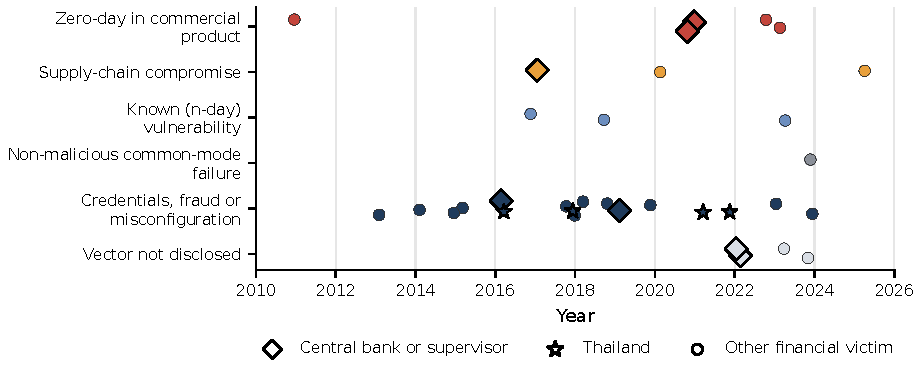
\includegraphics[width=\textwidth]{fig09_incidents.pdf}
\caption{Curated financial-sector incidents by year and initial-vector class. Diamonds: central banks or supervisors; stars: Thailand.}
\label{fig:incidents}
\end{figure}

Seven of the 33 cases hit central banks or supervisors. Their pattern is instructive: the RBNZ and EBA intrusions came through file-transfer and mail systems---commodity corporate IT---not through settlement systems. Bangladesh Bank was compromised in the environment around its payment-messaging interface. Bank Indonesia and the Bank of Zambia suffered ransomware.

\subsection{Would AI-discovered zero-days be used against banks?}
The evidence supports four statements. (i) Financial institutions are attractive targets for both financially motivated and state-linked actors. Some state-linked groups have a long record of attacks on banks and crypto firms (Bangladesh Bank, Bybit), and the AI-orchestrated campaign reported in 2025 reportedly included financial institutions among its intended targets \citep{anthropic2025espionage}. (ii) Zero-days reach banks through the commercial products that banks share with every other sector. An attacker does not need a ``banking zero-day''; an MFT or VPN zero-day reaches hundreds of banks at once. (iii) As AI lowers the cost of discovery, the scarcity that limited zero-day use to a few actors weakens. Mass-exploitation crews of the MOVEit type are the actors most likely to benefit, because their business model already converts one zero-day into many victims. (iv) We found no publicly documented case, up to our snapshot, of an AI-discovered zero-day used against a bank. Given the lags in public reporting and attackers' incentives not to disclose methods, this absence is weak evidence of safety.

\paragraph{Answer to RQ4.} The global banking system is exposed mainly through perimeter devices, MFT, IT-management tools, mail and collaboration servers, and shared service providers. AI-discovered zero-days are likely to be used against banks through these products. The likeliest form is mass exploitation and data extortion. Destructive attacks on payment systems are possible but less likely, because they require deeper access and invite a strong state response.
